In order to reduce the important number of tasks and communications, optimisations had to be applied at all levels of the algorithm. For that, we present in this section the evolution of the algorithm from the first natural version to the most optimized. As said in the section \ref{lu_algo}, the panel factorization is a loop of $n_b$ iterations. At each iteration $k$, several operations are executed on the panel.
The first natural version is that the node which contains the diagonal node compare progressively its maximum with others tiles. Each time it finds a better pivot, it saves it and uses it for next comparisons. After this operation, the task operating on the diagonal tile broadcasts the initial diagonal row and the selected row owning the column maximum to all others tiles in order that the concerned tile apply the swap, and every tile apply the \emph{scal} and \emph{ger} operations (Level 1 BLAS). Task flow~\ref{fig:natural_task_flow} shows one iteration of the panel factorization on a panel of 6 tiles for distributed architecture.

\begin{taskflow}[!ht]
\centering
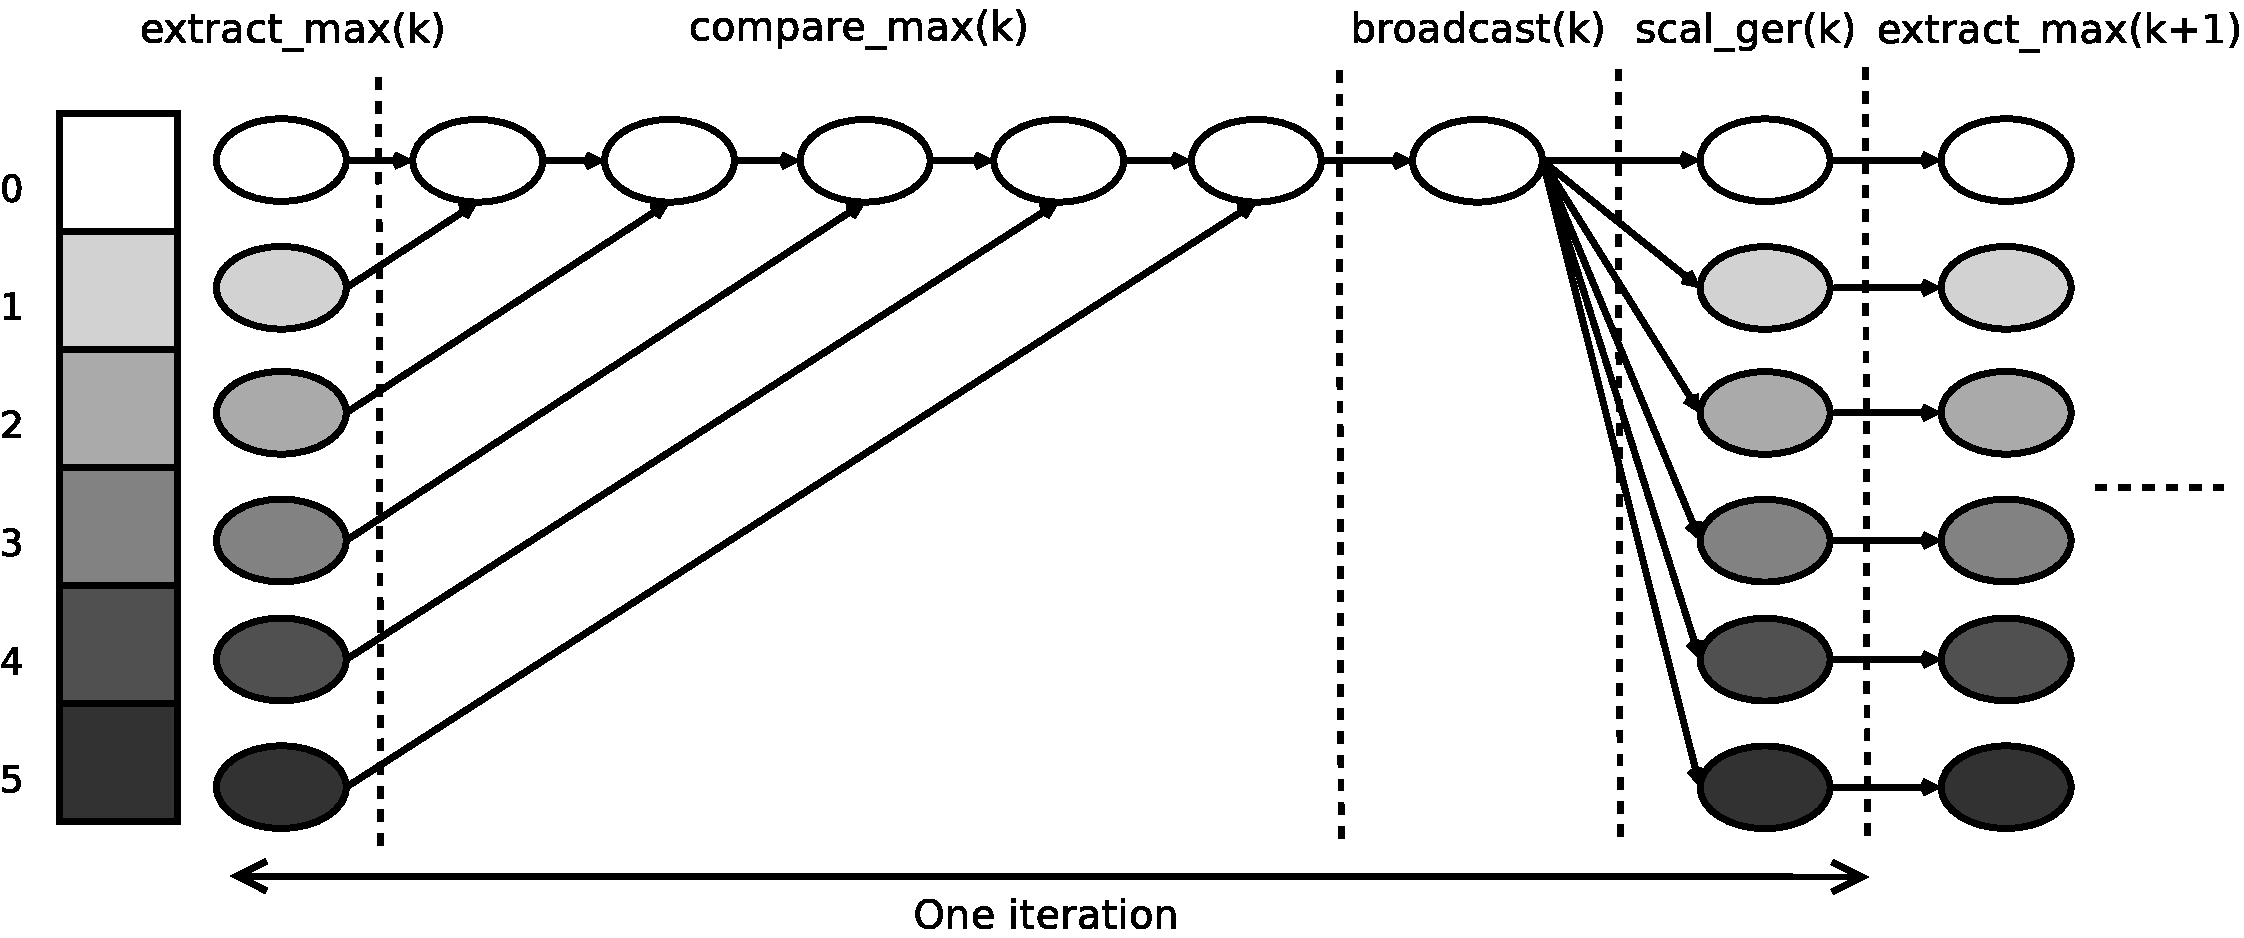
\includegraphics[width=0.8\textwidth]{figures/natural_tf_bw.pdf}
\caption{One iteration of panel factorization on distributed architecture \label{fig:natural_task_flow}}
\end{taskflow}

The first remark is that there are some communications which can be optimized. In fact, instead of using natural sequential comparison, it is possible to use a \emph{reduce} operation. It will allow to perform a faster election of the row owning the maximum of the column. Therefore, because the broadcast is following the operation of comparison, we can merge the two operations into one single \emph{all\_reduce} operation.
We can also merge tasks of extraction and tasks of panel update. For that, the \emph{extract\_max} of step $k$ and \emph{scal\_ger} of step $k-1$ tasks can be done in one single task.

Concerning communications, \dague and other runtimes handle point-to-point communications and can manage some collective communications as broadcast. But, to perform more complex communications operations (reduce, gather\dots), we have to express them as a task flow. 
%This is due to the programme model. In fact, a point-to-point communications or a broadcast are just a set of arrows between nodes of the PTG. 
This is due to the fact that reduce and/or gather operations are more complex to express with PTG and as of today are not available in the language used by \dague. For the \emph{all\_reduce} operation, the task flow needed is based on the task flow of the Bruck's algorithm \cite{BruckEtAl97}.
In the natural version, we broadcast two rows (the initial diagonal row and the selected row owning the maximum value of the column). Thus, for the \emph{all\_reduce} operation, an array of two rows per node is needed, we will call it a workspace. The first one is filled at beginning by the diagonal tile with the initial diagonal row, and the second row is filled by tasks operating on all panel tiles with the row holding the maximum value in the local column. At each step of the \textit{all\_reduce} operation, task copy first row from the received workspace if it is not empty, and reduce the seconds rows of the two workspaces according to the maximum value of their pivots. Thus, at the end of the \textit{all\_reduce} operation, all workspaces will be filled with the same values.
The resulting task flow is presented in Task flow \ref{fig:distributed_task_flow}.

\begin{taskflow}[!ht]
\centering
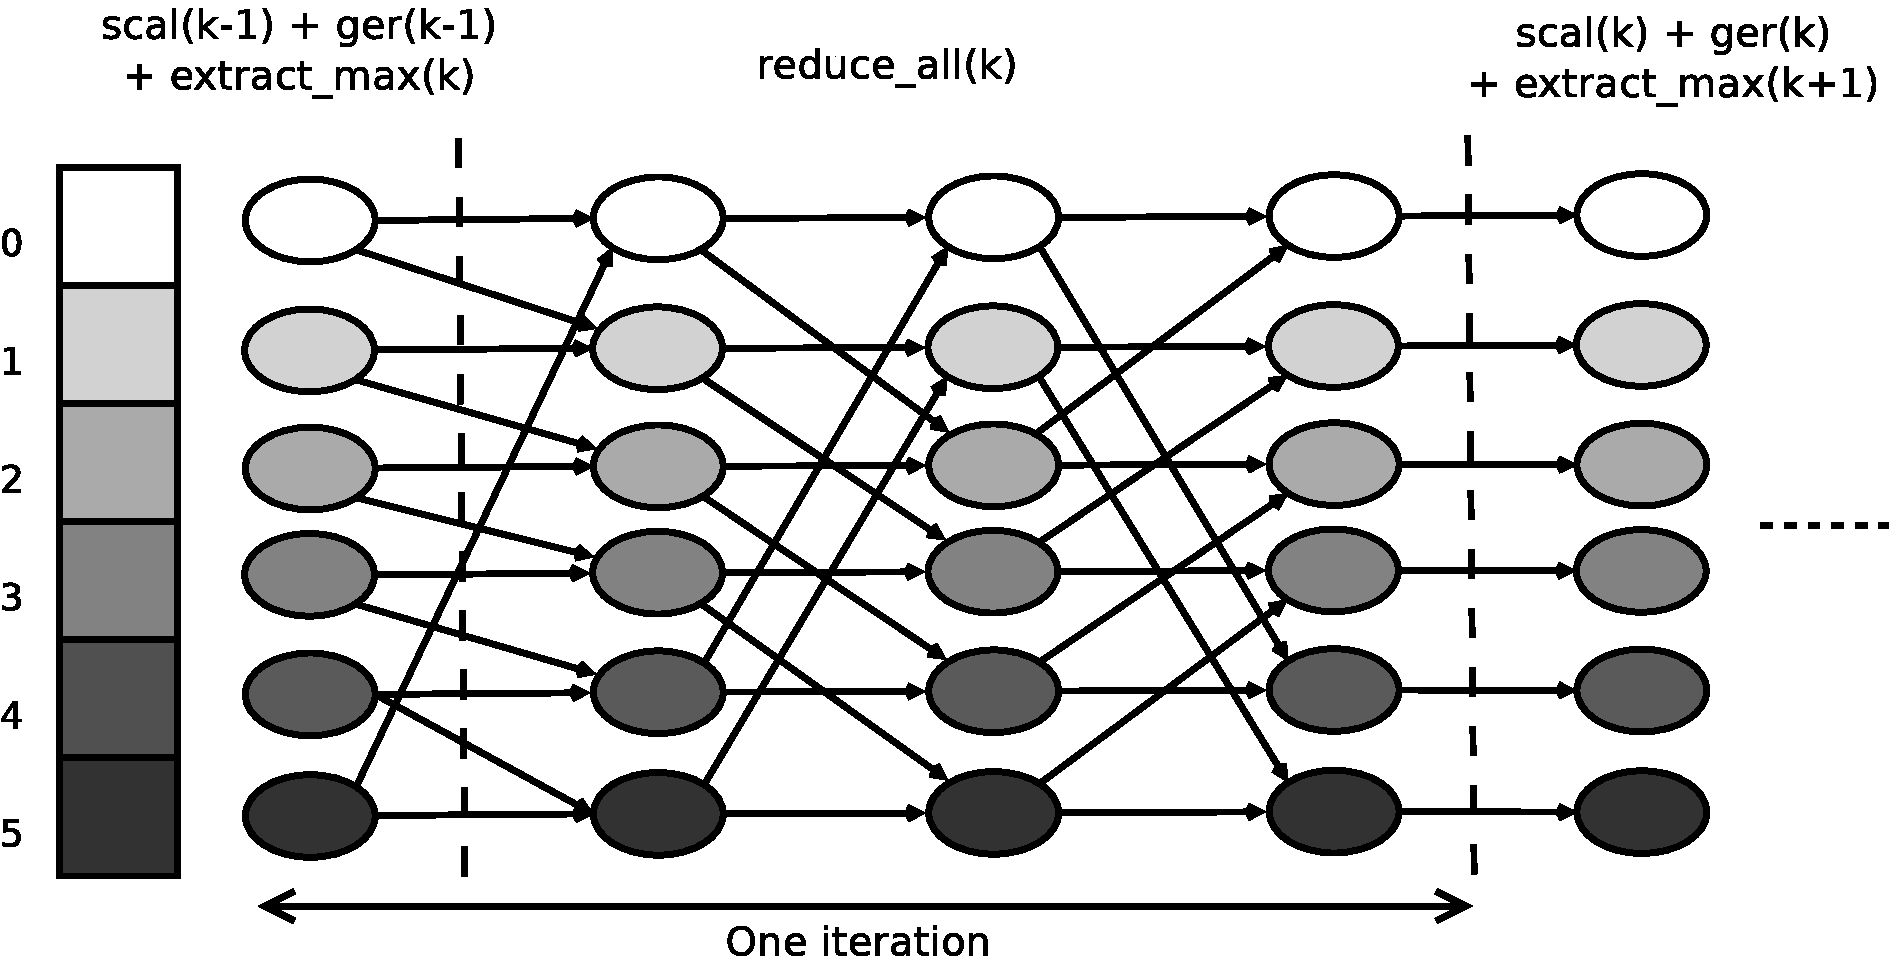
\includegraphics[width=0.6\textwidth]{figures/distributed_tf_bw.pdf}
\caption{One iteration of panel factorization on distributed architecture (combining reduce and broadcast communications)\label{fig:distributed_task_flow}}

\end{taskflow}

Nowadays, most distributed computers contain many cores at each node. To balance well the computations among the processors, a two-dimensional block-cyclic distribution is used to spread the data over the nodes\cite{DGW:SHPCC92}.
If we consider the fact that each node can be multi-core, the task flow \ref{fig:distributed_task_flow} can still be optimized. For that, the idea is to reduce first locally the maximum on the node and then, apply the \emph{all\_reduce} operation between the nodes. The \emph{reduce} operation is performed with a binary tree. Task flow \ref{fig:hybrid_task_flow} shows one iteration of panel factorization for hierarchical architecture. 

\begin{taskflow}[!ht]
\centering
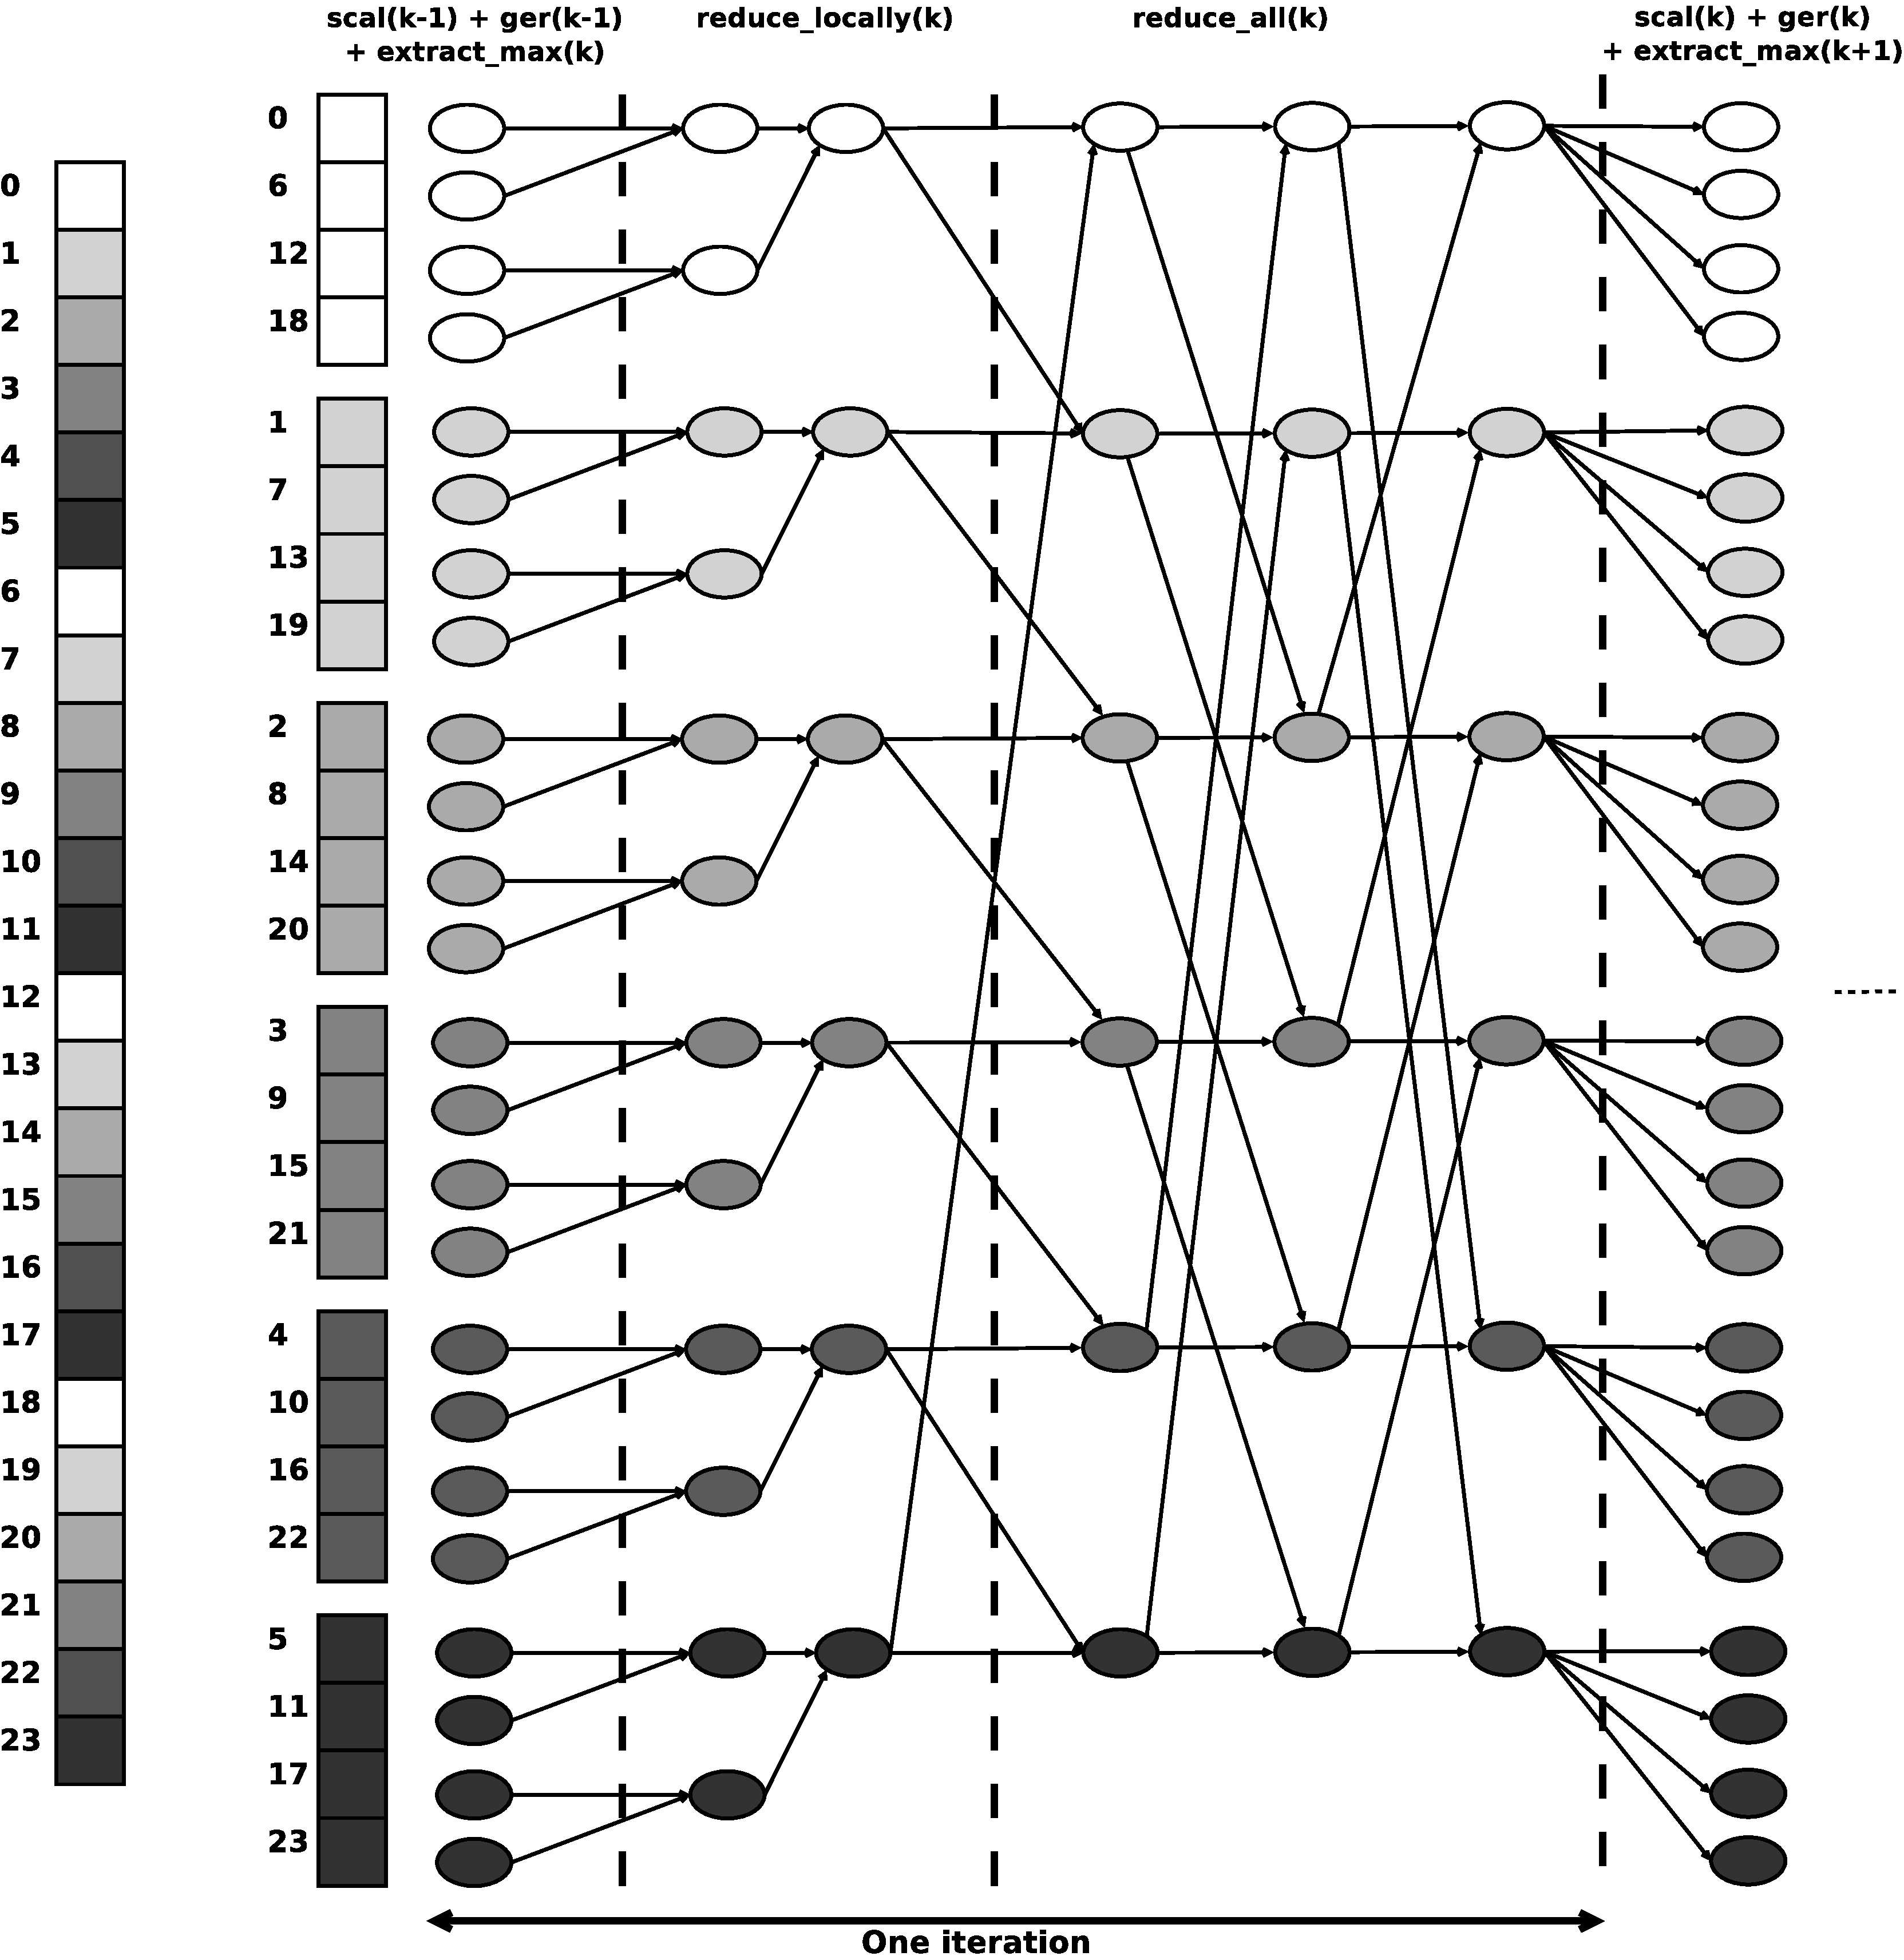
\includegraphics[width=0.7\textwidth]{figures/hybrid_tf_bw.pdf}
\caption{One iteration of panel factorization on hierarchical architecture \label{fig:hybrid_task_flow}}
\end{taskflow}
 
Whether in distributed, shared or hierarchical, the task flow showed in Task flows \ref{fig:natural_task_flow}, \ref{fig:distributed_task_flow} and \ref{fig:hybrid_task_flow} represent only one iteration of panel factorization. For the last iteration, an additional task is needed to finalize the panel factorization. In fact, this task perform the last \emph{scal} and \emph{ger} operations then release the dependencies to update the trailing sub-matrix.

Beside optimizations in task flow, we apply some optimization on kernel executed by tasks. In case of the task \textit{scal+ger+search\_max}, we use the notion of internal blocking. This optimization is the same applied from LINPACK to LAPACK libraries \cite{Anderson:1990:LPL}. Thanks to the internal blocking, we can use more Level 3 BLAS which increase the performance obtained. In fact, at each step of the panel factorization, instead applying \emph{ger} on the whole trailing sub-panel, we apply it only on a block. After each $ib$ iterations, $ib$ being the internal blocking parameter, the rest of the trailing sub-panel is updated by the level 3 BLAS operations \emph{trsm} and \emph{gemm} (Figure \ref{fig:panel_ib}).

\begin{figure}[!ht]
\centering
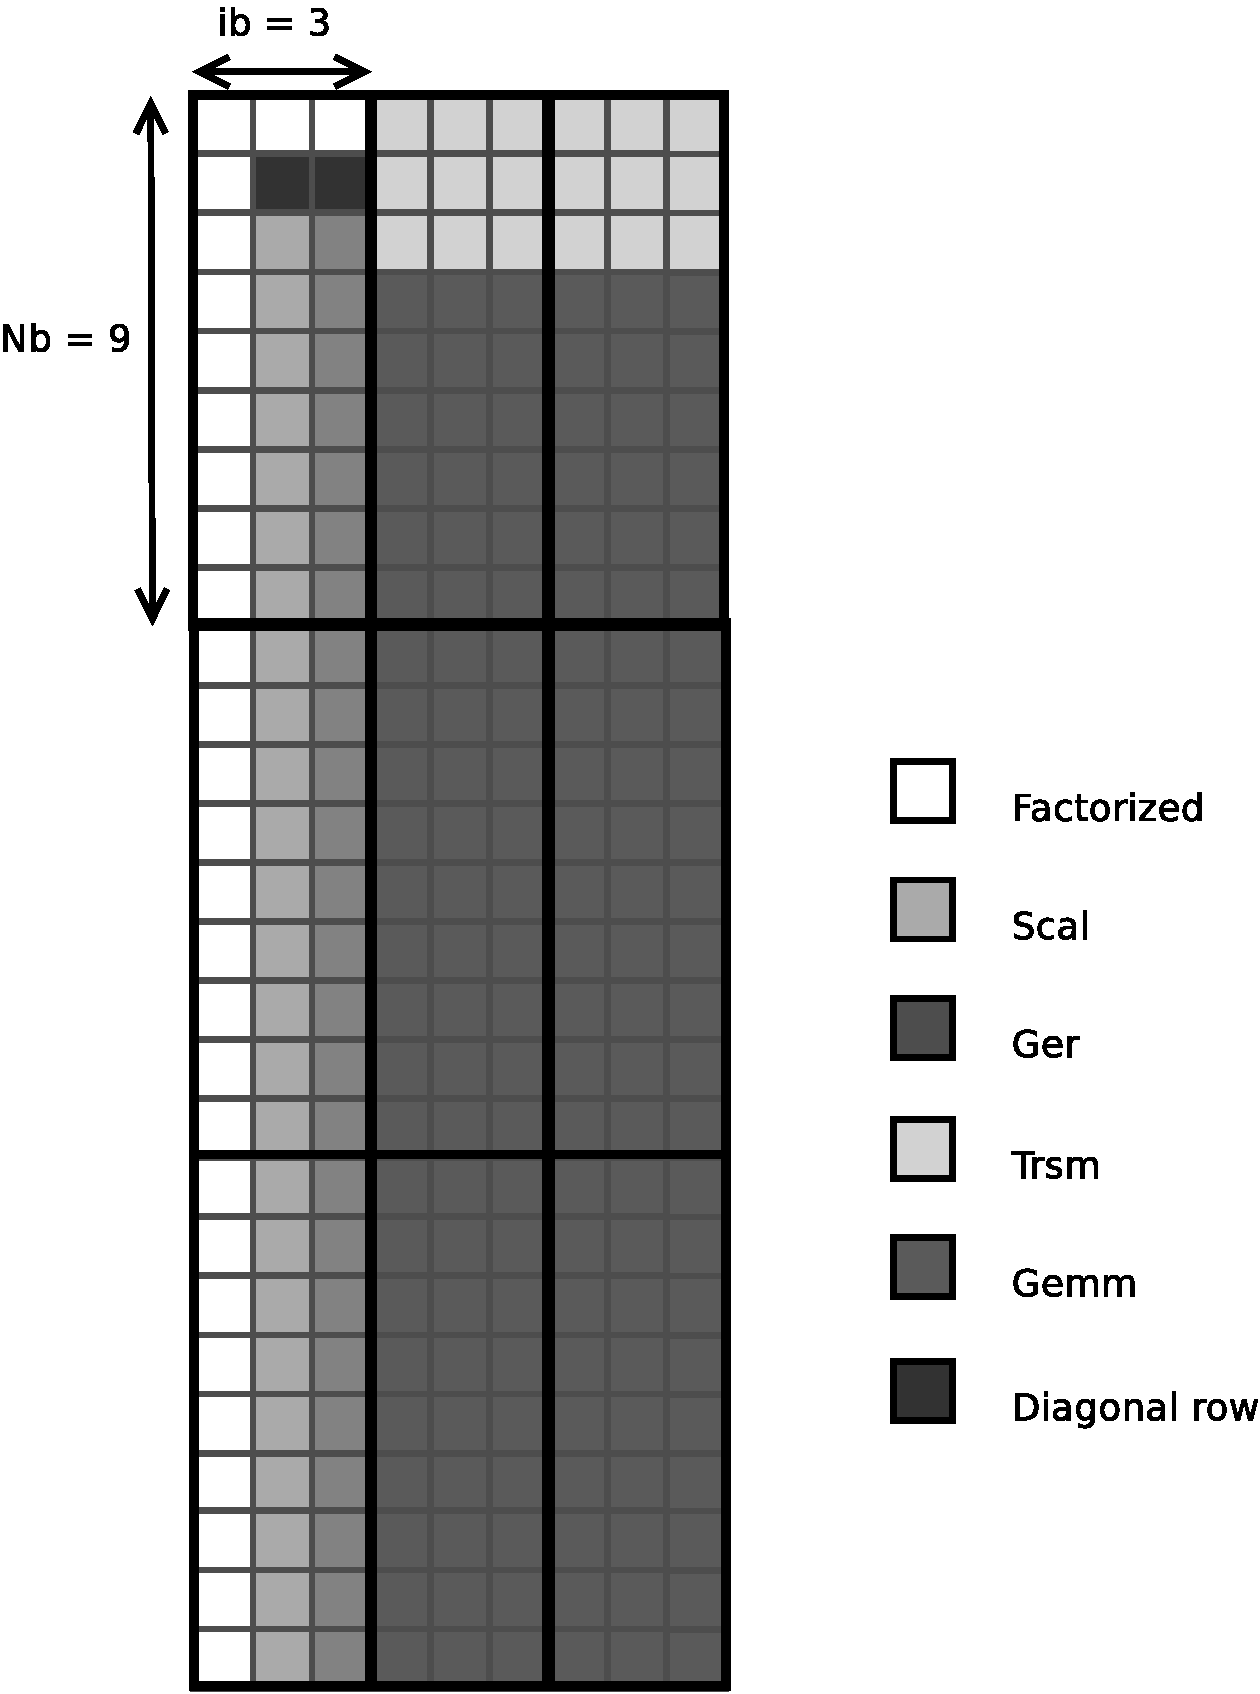
\includegraphics[height=8cm]{figures/panel_ib_bw.pdf}
\caption{Panel factorization with internal blocking\label{fig:panel_ib}}
\end{figure}
